\section{A Joint Model for Time-to-progression and Longitudinal Data}
\label{c1:sec:jm}
The first step in developing personalized schedules is processing a patient's surveillance data. This data includes baseline patient features, longitudinally measured outcomes of different types, and previous invasive test results. There are several challenges in modeling such data. First, longitudinal outcomes can be of different types (e.g., binary, continuous), are measured with error, and possibly correlated with each other. Second, usually, longitudinal measurements are not available after the patient is removed from surveillance upon observing progression. Third, patients who observe progression can have more adverse longitudinal data values. Fourth, time of progression is interval-censored (Figure~\ref{c1:fig:1}). Last, combining all this data to obtain a patient's personalized risk of progression. To overcome these challenges, we utilize the framework of joint models for time-to-event and longitudinal data~\citep{rizopoulos2012joint, tsiatis2004joint}.

\begin{figure}[tbp]
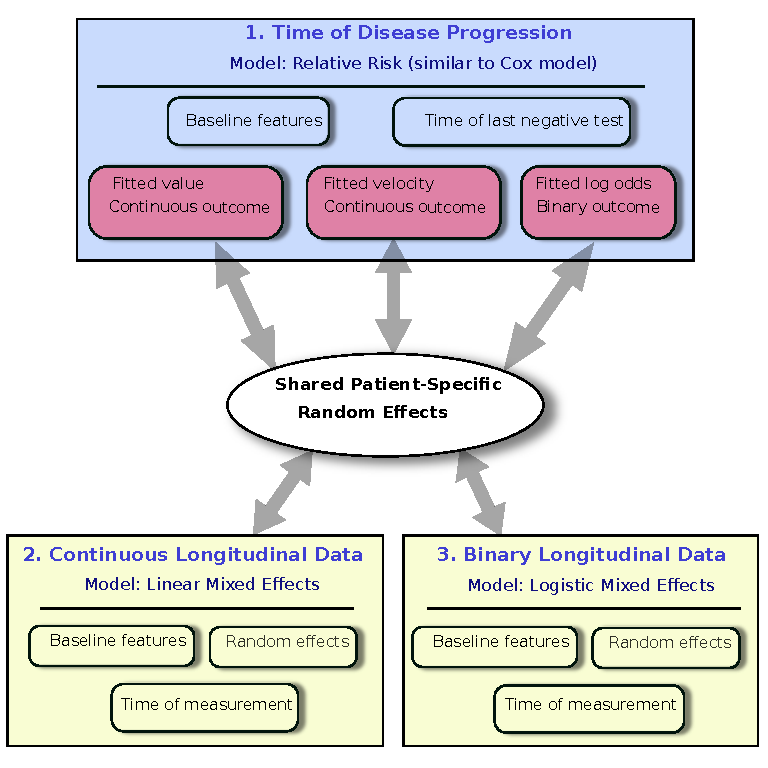
\includegraphics{contents/c1/images/c1_jm_blockdiag.pdf}
\caption{\textbf{Block diagram of a joint model for time-to-progression and longitudinal data}. Typically mixed effect sub-models are utilized for longitudinally measured data, and a relative-risk sub-model is employed for the interval-censored time of progression. The outcomes in these sub-models are conditionally independent of each other, given the common source of correlation patient-specific random-effects~\citep{laird1982random}. Different features of the longitudinal outcomes such as their fitted value, rate of change, fitted log-odds can be included in the relative-risk sub-model for predicting the risk of progression.} 
\label{c1:fig:c1_jm_blockdiag}
\end{figure}

The primary component in joint models is patient-specific random effects~\citep{laird1982random}. They represent the underlying state of disease, as well as act as the common source of correlation between different outcomes (Figure~\ref{c1:fig:c1_jm_blockdiag}) of a patient. Each outcome has a separate sub-model. Usually, mixed-effect sub-models are used for longitudinal outcomes, and a relative risk sub-model is employed for time-to-progression data. The parameters of the different sub-models are estimated jointly. Given a patient's data, the key output from the fitted joint model is a patient's personalized cumulative-risk of progression.

\subsection{Cumulative-risk of Progression}
Consider a joint model is fitted to a particular dataset. Given a new patient's accumulated data, the fitted joint model can predict his cumulative-risk of progression over his entire follow-up period starting from the time of his last negative test. This risk profile manifests the transition of a patient's disease state over time from low-risk to progressed. Hence, it can be used to guide the timing of invasive tests. In this regard, we have not only used the cumulative-risk to create personalized schedules but also for calculating a patient's expected time of progression. Although we estimate cumulative-risk using joint models, such estimates can also be obtained via other methods such as landmarking~\citep{hansVan2007dynamic}. In this regard, the scheduling methodology that we propose in this thesis is generic for use with any model that provides the cumulative-risk of progression.